\chapter{Supplementary Material}
\label{app:appendix-a}

\section{Project Timeline and Burndown}
\label{app:project-timeline-burndown}

\begin{figure}[H]
    \centering
    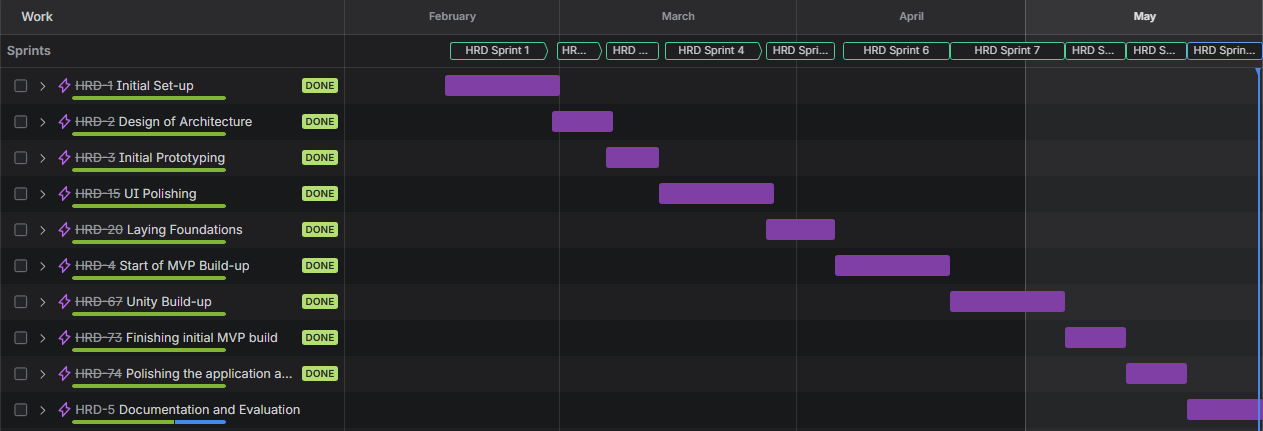
\includegraphics[width=\textwidth]{figures/project-timeline.png}
    \caption{Project timeline showing the main sprint periods and planned work items across the semester.}
    \label{fig:project-timeline}
\end{figure}

\begin{figure}[H]
    \centering
    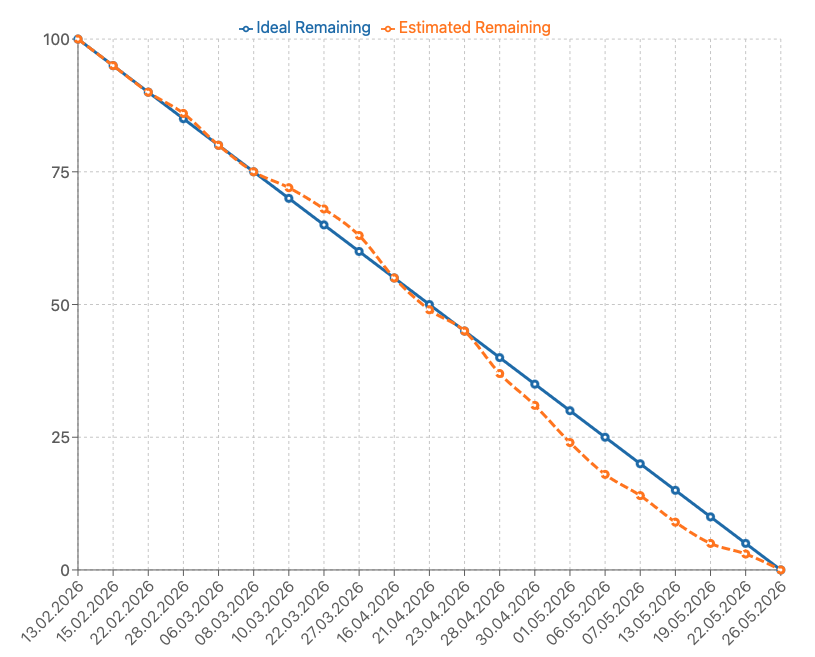
\includegraphics[width=0.85\textwidth]{figures/burndown-chart.png}
    \caption{Burndown chart comparing ideal remaining work with the estimated remaining work during the project.}
    \label{fig:burndown-chart}
\end{figure}

\section{Project Artefacts}
\label{app:project-artefacts}

The project source code is split into two repositories:

\begin{itemize}
    \item \textbf{Django backend and web dashboard:} \href{https://github.com/Ignat40/Bachelor-Thesis.git}{Ignat40/Bachelor-Thesis.git}
    \item \textbf{Unity mobile client:} \href{https://github.com/Rototype0/Phonemy-Client.git}{Rototype0/Phonemy-Client.git}
\end{itemize}
